\documentclass[12pt,a4paper]{article}

% ─── Page Layout ───────────────────────────────────────────────────────────────
\usepackage[a4paper, margin=0.8in, headheight=14pt]{geometry}

% ─── Fonts (XeLaTeX) ───────────────────────────────────────────────────────────
\usepackage{fontspec}
\usepackage{unicode-math}
\setmainfont{TeX Gyre Pagella}
\setmonofont[Scale=0.88]{TeX Gyre Cursor}
\setmathfont{Latin Modern Math}

% ─── Packages ──────────────────────────────────────────────────────────────────
\usepackage{xcolor}
\usepackage{colortbl}
\usepackage{titlesec}
\usepackage{enumitem}
\usepackage{tabularx}
\usepackage{booktabs}
\usepackage{array}
\usepackage{amsmath}
\usepackage{tikz}
\usetikzlibrary{shapes.geometric, arrows.meta, positioning, calc, fit, decorations.pathreplacing}
\usepackage{tcolorbox}
\tcbuselibrary{skins, breakable}
\usepackage{hyperref}
\usepackage{fancyhdr}
\usepackage{graphicx}
\usepackage{microtype}
\hyphenpenalty=10000
\exhyphenpenalty=10000
\sloppy
\usepackage{caption}
\usepackage{setspace}
\usepackage{multirow}
\usepackage{tocloft}

% ─── Q&A helper ────────────────────────────────────────────────────────────────
\newcommand{\Q}[1]{\textbf{#1}\par\noindent\ignorespaces}

% ─── Colour Palette ────────────────────────────────────────────────────────────
\definecolor{myred}{RGB}{196,30,58}
\definecolor{mydark}{RGB}{30,30,50}
\definecolor{mygreen}{RGB}{14,120,80}
\definecolor{myteal}{RGB}{0,130,140}
\definecolor{myamber}{RGB}{180,100,0}
\definecolor{mypurple}{RGB}{100,30,160}
\definecolor{mygray}{RGB}{246,247,249}
\definecolor{mgframe}{RGB}{180,185,200}
\definecolor{watermark}{RGB}{145,150,170}
\definecolor{hdrred}{RGB}{250,232,235}
\definecolor{hdrgreen}{RGB}{220,244,233}
\definecolor{hdrteal}{RGB}{220,242,244}
\definecolor{hdramber}{RGB}{253,242,215}
\definecolor{hdrpurple}{RGB}{238,228,255}
\definecolor{hdrgray}{RGB}{238,240,245}
\definecolor{rowalt}{RGB}{250,251,253}

% ─── Section Formatting ────────────────────────────────────────────────────────
\titleformat{\section}
  {\large\bfseries\color{myred}}{\thesection.}{0.5em}{}
  [\vspace{1pt}{\color{myred}\rule{\linewidth}{0.8pt}}]
\titleformat{\subsection}
  {\normalsize\bfseries\color{myteal}}{\thesubsection}{0.5em}{}
\titlespacing*{\section}{0pt}{18pt}{7pt}
\titlespacing*{\subsection}{0pt}{11pt}{4pt}

% ─── Paragraph ─────────────────────────────────────────────────────────────────
\setlength{\parindent}{0pt}
\setlength{\parskip}{4pt}

% ─── TOC Styling ───────────────────────────────────────────────────────────────
\renewcommand{\cfttoctitlefont}{\large\bfseries\color{myred}}
\renewcommand{\cftaftertoctitle}{\par\noindent{\color{myred}\rule{\linewidth}{0.8pt}}}
\setlength{\cftbeforetoctitleskip}{0pt}
\setlength{\cftaftertoctitleskip}{6pt}
\renewcommand{\cftsecfont}{\normalsize\bfseries\color{mydark}}
\renewcommand{\cftsecpagefont}{\normalsize\bfseries\color{mydark}}
\renewcommand{\cftsecleader}{\cftdotfill{\cftdotsep}}
\setlength{\cftbeforesecskip}{7pt}
\renewcommand{\cftsubsecfont}{\small\color{mydark}}
\renewcommand{\cftsubsecpagefont}{\small\color{mydark}}
\setlength{\cftbeforesubsecskip}{3pt}
\setlength{\cftsubsecindent}{1.4em}

% ─── Table helpers ─────────────────────────────────────────────────────────────
\renewcommand{\arraystretch}{1.45}
\setlength{\tabcolsep}{6pt}
\arrayrulecolor{mydark}
\newcolumntype{B}[1]{>{\small\bfseries\raggedright\arraybackslash}m{#1}}
\newcolumntype{Y}{>{\small\raggedright\arraybackslash}X}
\renewcommand{\tabularxcolumn}[1]{m{#1}}

% ─── Header / Footer ───────────────────────────────────────────────────────────
\pagestyle{fancy}
\fancyhf{}
\fancyhead[L]{\small\color{myred}\textbf{PE-EC603B}\;\color{mydark}--- Bio-Medical Electronics}
\fancyhead[R]{\small\color{myteal}\textbf{Module 2 Notes}}
\fancyfoot[C]{\small\color{mydark}\thepage}
\fancyfoot[R]{\small\color{watermark}\textit{\copyright\ Biraj}}
\renewcommand{\headrulewidth}{0.5pt}
\renewcommand{\footrulewidth}{0.3pt}

% ─── Hyperref ──────────────────────────────────────────────────────────────────
\hypersetup{
  colorlinks=true, linkcolor=myteal, urlcolor=myteal,
  pdfauthor={Biraj Sarkar},
  pdftitle={PE-EC603B --- Module 2 Notes}
}

% ─── tcolorbox styles ──────────────────────────────────────────────────────────
\tcbset{
  tikzbox/.style={
    colback=mygray, colframe=mgframe, boxrule=0.6pt, arc=4pt,
    left=8pt, right=8pt, top=6pt, bottom=6pt,
    colbacktitle=mgframe, coltitle=mydark,
    fonttitle=\small\bfseries
  },
  defbox/.style={
    colback=hdrgreen, colframe=mygreen, boxrule=0.8pt, arc=4pt,
    left=9pt, right=9pt, top=6pt, bottom=6pt,
    colbacktitle=mygreen, coltitle=white,
    fonttitle=\small\bfseries
  },
  formulabox/.style={
    colback=hdrteal, colframe=myteal, boxrule=0.8pt, arc=4pt,
    left=9pt, right=9pt, top=7pt, bottom=7pt,
    colbacktitle=myteal, coltitle=white,
    fonttitle=\small\bfseries
  },
  examplebox/.style={
    colback=hdramber, colframe=myamber, boxrule=0.8pt, arc=4pt,
    left=9pt, right=9pt, top=6pt, bottom=6pt,
    colbacktitle=myamber, coltitle=white,
    fonttitle=\small\bfseries
  },
  masonbox/.style={
    colback=hdrpurple, colframe=mypurple, boxrule=0.8pt, arc=4pt,
    left=9pt, right=9pt, top=6pt, bottom=6pt,
    colbacktitle=mypurple, coltitle=white,
    fonttitle=\small\bfseries
  },
  exambox/.style={
    colback=hdrpurple, colframe=mypurple, boxrule=1pt, arc=5pt,
    left=10pt, right=10pt, top=8pt, bottom=8pt,
    colbacktitle=mypurple, coltitle=white,
    fonttitle=\bfseries,
    breakable, title after break={\textbf{Frequently Asked / Viva Questions (contd.)}}}
}
\tcbset{breakable}

% ─── TikZ styles ───────────────────────────────────────────────────────────────
\tikzset{
  block/.style={rectangle, draw=myteal, fill=hdrteal,
    text width=2.4cm, align=center, minimum height=0.95cm,
    font=\small, rounded corners=3pt, line width=0.7pt},
  redblock/.style={rectangle, draw=myred, fill=hdrred,
    text width=2.4cm, align=center, minimum height=0.95cm,
    font=\small, rounded corners=3pt, line width=0.7pt},
  greenblock/.style={rectangle, draw=mygreen, fill=hdrgreen,
    text width=2.4cm, align=center, minimum height=0.95cm,
    font=\small, rounded corners=3pt, line width=0.7pt},
  amberblock/.style={rectangle, draw=myamber, fill=hdramber,
    text width=2.4cm, align=center, minimum height=0.95cm,
    font=\small, rounded corners=3pt, line width=0.7pt},
  purpblock/.style={rectangle, draw=mypurple, fill=hdrpurple,
    text width=2.4cm, align=center, minimum height=0.95cm,
    font=\small, rounded corners=3pt, line width=0.7pt},
  sumjunc/.style={circle, draw=myamber, fill=hdramber,
    minimum size=0.62cm, font=\small, line width=0.8pt},
  arrow/.style={-Stealth, thick, color=mydark},
  redarrow/.style={-Stealth, thick, color=myred},
  line/.style={thick, color=mydark}
}

% ═══════════════════════════════════════════════════════════════════════════════
\begin{document}
% ═══════════════════════════════════════════════════════════════════════════════

\begin{center}
  {\LARGE\bfseries\color{myred} PE-EC603B --- Bio-Medical Electronics}\\[5pt]
  {\normalsize\color{mydark} Semester VI \quad$\bullet$\quad 3L:0T:0P \quad$\bullet$\quad 3 Credits}\\[3pt]
  {\normalsize\color{myteal}\textbf{Module 2 Exam Notes: Biomedical Transducers and Bio-potential Amplifiers}}\\[3pt]
  {\small\color{mydark} CGEC \;$|$\; B.Tech ECE (2023--27) \;$|$\; \textit{Biraj Sarkar}}
\end{center}
\vspace{2pt}
\noindent{\color{myred}\rule{\linewidth}{1.5pt}}
\vspace{2pt}

\hypersetup{linkcolor=mydark}
\tableofcontents
\hypersetup{linkcolor=myteal}
\newpage

% ===============================================================================
\section{Biomedical Transducers --- Classification and Characteristics}
% ===============================================================================

\begin{tcolorbox}[defbox, title={\textbf{Definition: Biomedical Transducer}}]
A \textbf{biomedical transducer} is a device that converts a physiological (biological or physical) variable into an electrical signal suitable for measurement, display, recording, or processing. It acts as the primary sensing element in a medical instrument.
\end{tcolorbox}

\subsection{Classification of Biomedical Transducers}

\textbf{1. By Transduction Principle:}\par\noindent
\begin{tabularx}{\linewidth}{|B{3.0cm}|Y|Y|}
\hline
\textbf{Type} & \textbf{\color{myteal}Principle} & \textbf{\color{mygreen}Example} \\
\hline
\textbf{Resistive} & Measured quantity changes resistance. & Strain gauge, thermistor, potentiometer. \\
\hline
\textbf{Capacitive} & Measured quantity changes capacitance. & Capacitive pressure sensor, microphone. \\
\hline
\textbf{Inductive / LVDT} & Movement changes mutual inductance. & LVDT (Linear Variable Differential Transformer). \\
\hline
\textbf{Piezoelectric} & Mechanical stress produces a voltage. & Ultrasonic transducer, force sensor. \\
\hline
\textbf{Photoelectric} & Light intensity changes output current. & Pulse oximeter, photodiode sensor. \\
\hline
\textbf{Electrochemical} & Ion concentration generates EMF. & pH electrode, ion-selective electrode. \\
\hline
\textbf{Thermoelectric} & Temperature difference generates voltage. & Thermocouple (Seebeck effect). \\
\hline
\end{tabularx}

\textbf{2. By Input Quantity:} Displacement, Velocity, Force, Pressure, Acceleration, Flow, Temperature, Potential, Chemical concentration.

\subsection{Desirable Characteristics of a Biomedical Transducer}

\begin{itemize}[leftmargin=*, itemsep=3pt]
  \item \textbf{High Sensitivity:} Large output per unit physiological change.
  \item \textbf{High Linearity:} Output proportional to input over the full range.
  \item \textbf{Low Hysteresis:} Output should not depend on direction of change.
  \item \textbf{High Signal-to-Noise Ratio (SNR):} Minimum interference and noise pick-up.
  \item \textbf{Biocompatibility:} Non-toxic, non-irritating, and chemically inert when implanted or in contact with tissue.
  \item \textbf{Minimal Loading Effect:} The transducer should not disturb the physiological system it is measuring.
  \item \textbf{Stability and Reproducibility:} Consistent readings over time and repeated measurements.
\end{itemize}

% ===============================================================================
\section{Displacement and Velocity Transducers}
% ===============================================================================

\subsection{Strain Gauge (Resistive)}

\begin{tcolorbox}[defbox, title={\textbf{Strain Gauge}}]
A \textbf{strain gauge} is a resistive sensor whose electrical resistance changes proportionally to the mechanical strain (deformation) applied to it. Used to measure force, pressure, torque, and displacement indirectly.
\end{tcolorbox}

\begin{tcolorbox}[formulabox, title={\textbf{Strain Gauge Formula}}]
\[
\frac{\Delta R}{R} = G_F \cdot \varepsilon
\]
where $\varepsilon = \dfrac{\Delta L}{L}$ is the mechanical strain, and $G_F$ is the \textbf{Gauge Factor} (typically $2$ for metal foil gauges; up to $150$ for semiconductor gauges).
\[
G_F = \frac{\Delta R/R}{\varepsilon} = 1 + 2\nu + \pi_\ell E
\]
$\nu$ = Poisson's ratio; $\pi_\ell$ = piezoresistive coefficient; $E$ = Young's modulus.
\end{tcolorbox}

Strain gauges are arranged in a \textbf{Wheatstone bridge} to improve sensitivity and temperature compensation. For blood pressure measurement, the strain gauge is bonded to a stainless steel diaphragm.

\subsection{LVDT (Linear Variable Differential Transformer)}

\begin{tcolorbox}[defbox, title={\textbf{LVDT}}]
The \textbf{Linear Variable Differential Transformer (LVDT)} is an inductive displacement sensor that produces an AC voltage output proportional to the linear displacement of a movable ferromagnetic core.
\end{tcolorbox}

\begin{tcolorbox}[tikzbox, title={LVDT Schematic Diagram}]
\centering
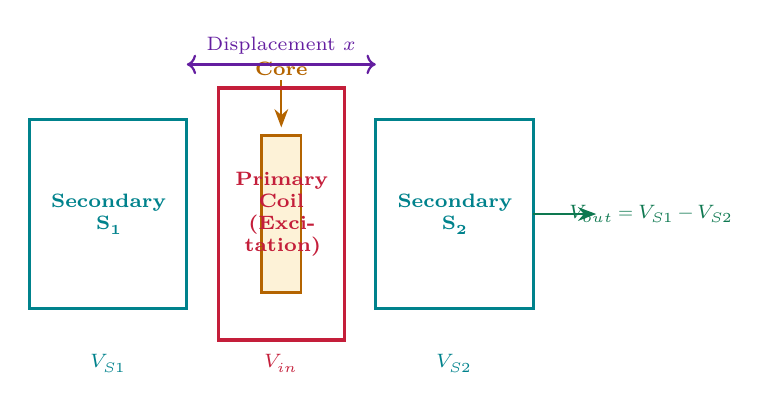
\begin{tikzpicture}[thick, font=\small]
  % Core (movable)
  \filldraw[fill=hdramber, draw=myamber, line width=1pt] (0.55, 0.6) rectangle (1.05, 2.6);
  \node[color=myamber, font=\scriptsize\bfseries] at (0.8, 3.45) {Core};
  \draw[arrow, color=myamber] (0.8, 3.3) -- (0.8, 2.7);

  % Primary coil (centre)
  \draw[color=myred, line width=1.2pt] (0, 0) rectangle (1.6, 3.2);
  \node[color=myred, font=\scriptsize\bfseries, align=center, text width=1.5cm] at (0.8, 1.6) {Primary\\Coil\\(Excitation)};

  % Secondary coil S1 (left)
  \draw[color=myteal, line width=1.2pt] (-2.4, 0.4) rectangle (-0.4, 2.8);
  \node[color=myteal, font=\scriptsize\bfseries, align=center, text width=1.5cm] at (-1.4, 1.6) {Secondary\\S\textsubscript{1}};

  % Secondary coil S2 (right)
  \draw[color=myteal, line width=1.2pt] (2.0, 0.4) rectangle (4.0, 2.8);
  \node[color=myteal, font=\scriptsize\bfseries, align=center, text width=1.5cm] at (3.0, 1.6) {Secondary\\S\textsubscript{2}};

  % Displacement arrow
  \draw[<->, color=mypurple, thick] (-0.4, 3.5) -- (2.0, 3.5) node[midway, above, font=\scriptsize, color=mypurple] {Displacement $x$};

  % Output labels
  \node[font=\scriptsize, color=myteal] at (-1.4, -0.3) {$V_{S1}$};
  \node[font=\scriptsize, color=myteal] at (3.0, -0.3) {$V_{S2}$};
  \node[font=\scriptsize, color=myred] at (0.8, -0.3) {$V_{in}$};
  \node[font=\scriptsize, color=mygreen] at (5.5, 1.6) {$V_{out} = V_{S1} - V_{S2}$};
  \draw[arrow, color=mygreen] (4.0, 1.6) -- (4.8, 1.6);
\end{tikzpicture}
\end{tcolorbox}

\textbf{Working:} When the core is at the centre (null position), $V_{S1} = V_{S2}$, so $V_{out} = 0$. Displacement to one side increases coupling to that secondary coil, creating a differential output proportional to displacement. The output phase indicates direction of displacement.

\textbf{Biomedical Applications:} Measuring chest wall movement during respiration, arterial diameter pulsation, bone growth measurement.

% ===============================================================================
\section{Force, Pressure, and Acceleration Transducers}
% ===============================================================================

\subsection{Piezoelectric Transducer}

\begin{tcolorbox}[defbox, title={\textbf{Piezoelectric Effect}}]
The \textbf{piezoelectric effect} is the generation of an electric charge on certain crystalline materials (e.g., quartz, PZT --- Lead Zirconate Titanate, PVDF) when they are subjected to mechanical stress or deformation. Conversely, an applied electric field causes the material to deform (\textbf{converse piezoelectric effect}).
\end{tcolorbox}

\begin{tcolorbox}[formulabox, title={\textbf{Piezoelectric Sensor Equations}}]
\[
Q = d_{ij} \cdot F \qquad V_{out} = \frac{Q}{C_p} = \frac{d_{ij} \cdot F}{C_p}
\]
where $Q$ = generated charge (C), $d_{ij}$ = piezoelectric charge constant (C/N), $F$ = applied force (N), $C_p$ = sensor capacitance (F). \\[4pt]
Sensitivity: $S = \dfrac{V_{out}}{F} = \dfrac{d_{ij}}{C_p}$ \quad (V/N)
\end{tcolorbox}

\textbf{Biomedical Applications:} Ultrasonic imaging transducers (transmit and receive), phonocardiography (heart sound recording), pulse waveform measurement, bone conduction hearing aids.

\textbf{Limitations:} Cannot measure static forces (DC signals bleed away through parasitic resistance). Requires high-input-impedance amplifiers.

\subsection{Capacitive Pressure Sensor}

A capacitive pressure sensor uses a flexible diaphragm as one plate of a capacitor. Applied pressure deflects the diaphragm, changing the gap $d$:
\[
C = \frac{\varepsilon_0 \varepsilon_r A}{d} \qquad \Rightarrow \qquad \Delta C \propto \Delta P
\]
Used in blood pressure catheters, intra-cranial pressure (ICP) monitoring.

\subsection{Accelerometer}

\begin{tcolorbox}[defbox, title={\textbf{Accelerometer}}]
An \textbf{accelerometer} is a transducer that measures acceleration (rate of change of velocity), typically based on a proof mass attached to a spring-damper system. Used to assess patient movement, gait analysis, and in implantable cardiac pacemakers (rate-responsive pacing).
\end{tcolorbox}

$F = ma \Rightarrow$ deflection of mass proportional to acceleration. Piezoresistive or capacitive sensing of the deflection gives output voltage $\propto$ acceleration.

% ===============================================================================
\section{Flow and Temperature Transducers}
% ===============================================================================

\subsection{Electromagnetic Blood Flow Transducer}

\begin{tcolorbox}[defbox, title={\textbf{Electromagnetic Flowmeter}}]
Based on \textbf{Faraday's law of electromagnetic induction}: when a conductor (blood, which contains ions) moves through a magnetic field, an EMF is induced perpendicular to both the flow direction and the magnetic field.
\end{tcolorbox}

\begin{tcolorbox}[formulabox, title={\textbf{Electromagnetic Flowmeter Formula}}]
\[
V_{emf} = B \cdot d \cdot v
\]
where $B$ = magnetic flux density (T), $d$ = inner diameter of vessel (m), $v$ = mean blood velocity (m/s). \\[4pt]
Volumetric Flow Rate: $Q = v \cdot A = v \cdot \dfrac{\pi d^2}{4}$
\end{tcolorbox}

\textbf{Advantages:} No obstruction to flow, direct velocity measurement, works with pulsatile flow. \textbf{Limitation:} Requires surgical placement around the vessel (perivascular cuff type).

\subsection{Ultrasonic (Doppler) Flow Transducer}

When ultrasound is transmitted into blood and reflected from moving red blood cells, the reflected frequency is shifted:
\[
\Delta f = f_r - f_t = \frac{2 f_t \cdot v \cdot \cos\theta}{c}
\]
where $v$ = blood velocity, $\theta$ = angle between ultrasound beam and flow direction, $c$ = speed of sound in tissue ($\approx 1540\,\text{m/s}$). \\[4pt]
Non-invasive, used in vascular Doppler studies and echocardiography.

\subsection{Temperature Transducers}

\par\noindent
\begin{tabularx}{\linewidth}{|B{2.8cm}|Y|>{\centering\arraybackslash}m{2.0cm}|Y|}
\hline
\textbf{Type} & \textbf{\color{myteal}Principle} & \textbf{\color{myamber}Range} & \textbf{\color{mygreen}Biomedical Use} \\
\hline
\textbf{Thermistor} & NTC/PTC semiconductor resistance vs.\ temperature. & $-50$ to $150\,^{\circ}$C & Rectal/skin/blood temp. \\
\hline
\textbf{Thermocouple} & Seebeck effect: voltage at junction of dissimilar metals. & $-200$ to $1200\,^{\circ}$C & Surgical probes, cryosurgery. \\
\hline
\textbf{RTD (Pt100)} & Platinum resistance increases linearly with temperature. & $-200$ to $600\,^{\circ}$C & Precision lab instruments. \\
\hline
\textbf{IC Sensor} & Semiconductor bandgap vs.\ temperature (e.g., LM35). & $-55$ to $150\,^{\circ}$C & Clinical thermometers. \\
\hline
\end{tabularx}

\textbf{Thermistor Equation (NTC):}
\[
R_T = R_0 \cdot e^{B\left(\frac{1}{T} - \frac{1}{T_0}\right)}
\]
where $B$ = material constant ($2000$--$5000\,\text{K}$), $T$ = temperature in Kelvin, $R_0$ = resistance at reference temperature $T_0$.

% ===============================================================================
\section{Chemical and Ion-Selective Transducers}
% ===============================================================================

\begin{tcolorbox}[defbox, title={\textbf{Ion-Selective Electrode (ISE)}}]
An \textbf{ion-selective electrode} generates a potential proportional to the logarithm of the concentration of a specific ion (e.g., $\text{Na}^+$, $\text{K}^+$, $\text{Ca}^{2+}$, $\text{H}^+$) in the solution according to the \textbf{Nernst equation}.
\end{tcolorbox}

\begin{tcolorbox}[formulabox, title={\textbf{Nernst Equation and pH Electrode}}]
\[
E = E^0 + \frac{RT}{zF}\ln[\text{ion}] \quad = E^0 - \frac{0.0592}{z}\log[\text{ion}] \quad \text{(at } 25\,^{\circ}\text{C)}
\]
For \textbf{pH electrode} ($z=1$ for H\textsuperscript{+}): $E = E^0 - 59.2\,\text{mV} \times \text{pH}$ \quad (Sensitivity: $59.2\,\text{mV/pH}$)
\end{tcolorbox}

\textbf{Dissolved Gas Sensors:}
\begin{itemize}[leftmargin=*, itemsep=3pt]
  \item \textbf{Clark Electrode (pO\textsubscript{2}):} Amperometric sensor. O\textsubscript{2} is reduced at a platinum cathode through a semipermeable membrane; current is proportional to $\text{pO}_2$.
  \item \textbf{Severinghaus Electrode (pCO\textsubscript{2}):} CO\textsubscript{2} diffuses through a membrane into bicarbonate solution, changing its pH, measured by a pH electrode.
\end{itemize}

% ===============================================================================
\section{Bio-electrodes}
% ===============================================================================

\begin{tcolorbox}[defbox, title={\textbf{Bio-electrode}}]
A \textbf{bio-electrode} is an interface between the biological medium (ionic conduction) and the measurement circuitry (electronic conduction). It converts ionic current flow in tissues to electron current flow in metallic wires.
\end{tcolorbox}

\subsection{Electrode--Electrolyte Interface and Half-Cell Potential}

At the electrode--electrolyte interface, oxidation/reduction reactions create a \textbf{half-cell potential} $E_{HC}$. For a metal electrode:
\[
M \rightleftharpoons M^{n+} + ne^- \qquad E_{HC} = E^0 + \frac{RT}{nF}\ln[M^{n+}]
\]
The \textbf{electrode offset potential} creates a DC bias that can saturate amplifiers if not accounted for.

\subsection{Types of Electrodes}

\par\noindent
\begin{tabularx}{\linewidth}{|B{2.8cm}|Y|Y|}
\hline
\textbf{Type} & \textbf{\color{myteal}Description} & \textbf{\color{mygreen}Application} \\
\hline
\textbf{Ag/AgCl Surface} & Silver coated with AgCl paste; very stable, low offset potential. & Standard ECG chest electrodes, EEG. \\
\hline
\textbf{Carbon / Paste} & Conductive carbon paste; disposable, low cost. & Holter monitor, disposable ECG patches. \\
\hline
\textbf{Needle Electrode} & Fine steel or platinum needle inserted into muscle. & Clinical EMG recording, nerve conduction. \\
\hline
\textbf{Concentric Needle} & Inner wire in insulated cannula; records single motor unit. & Single motor unit EMG. \\
\hline
\textbf{Floating Electrode} & Electrode body floats; electrolyte gel bridges skin. & Long-term ambulatory monitoring. \\
\hline
\textbf{Suction Electrode} & Adheres to skin via suction (no adhesive). & Chest ECG, temporary use. \\
\hline
\textbf{Microelectrode} & Glass capillary filled with KCl; tip $< 1\,\mu\text{m}$. & Intracellular recording of action potentials. \\
\hline
\end{tabularx}

\textbf{Equivalent circuit of a bio-electrode:} Series combination of half-cell potential $E_{HC}$, electrode resistance $R_e$, and double-layer capacitance $C_d$, in series with the tissue resistance $R_t$.

% ===============================================================================
\section{Bio-potential Amplifiers and Signals}
% ===============================================================================

\subsection{Requirements of a Bio-potential Amplifier}

Bio-electrical signals (ECG, EMG, EEG) have very small amplitudes ($\mu$V to mV range) contaminated by electrode offset potentials, motion artefacts, and 50/60 Hz power-line interference. A bio-potential amplifier must have:

\begin{itemize}[leftmargin=*, itemsep=3pt]
  \item \textbf{Very High Input Impedance} ($> 10\,\text{M}\Omega$): To minimize loading of the high-impedance electrode--skin interface.
  \item \textbf{High Common Mode Rejection Ratio (CMRR)} ($> 80\,\text{dB}$): To reject the 50 Hz power-line interference which appears as a common-mode signal on both input electrodes.
  \item \textbf{Low Noise:} Input-referred noise $< 1\,\mu\text{V}_{rms}$ for EEG.
  \item \textbf{High Gain:} Sufficient to bring signals to ADC-compatible levels (typically $\times 1000$).
  \item \textbf{Appropriate Bandwidth:} ECG: $0.05$--$150\,\text{Hz}$; EMG: $5$--$2000\,\text{Hz}$; EEG: $0.5$--$100\,\text{Hz}$.
  \item \textbf{Patient Safety Isolation:} Galvanic isolation (optocouplers or transformers) to prevent micro-shock from leakage currents.
\end{itemize}

\subsection{Instrumentation Amplifier (INA)}

The \textbf{instrumentation amplifier (INA)} is the standard front-end for bio-potential amplifiers. It consists of three op-amps:

\begin{tcolorbox}[tikzbox, title={3-Op-Amp Instrumentation Amplifier Block Diagram}]
\centering
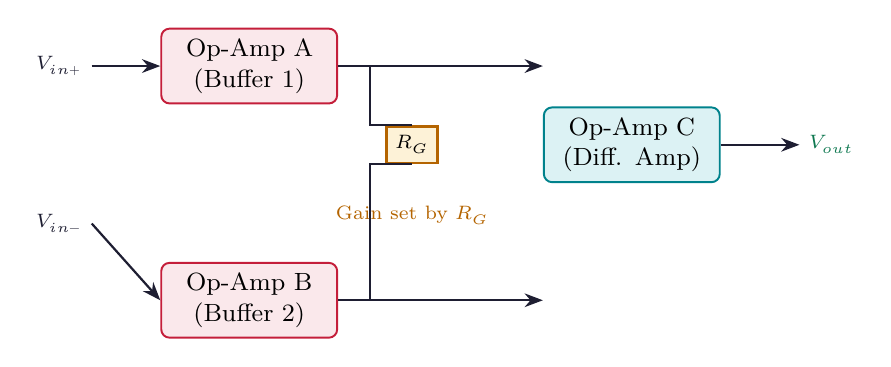
\begin{tikzpicture}[node distance=1.2cm and 2.2cm, thick, font=\small]
  % Input buffer op-amps
  \node[redblock, text width=2.0cm] (opA) {Op-Amp A\\(Buffer 1)};
  \node[redblock, text width=2.0cm, below=2.0cm of opA] (opB) {Op-Amp B\\(Buffer 2)};
  \node[block, text width=2.0cm, right=2.6cm of opA, yshift=-1.0cm] (opC) {Op-Amp C\\(Diff. Amp)};

  % Resistor Rg
  \node[draw=myamber, fill=hdramber, minimum width=0.6cm, minimum height=0.35cm,
        font=\scriptsize, right=0.6cm of opA, yshift=-1.0cm] (Rg) {$R_G$};

  % Input labels
  \draw[arrow] (-2.0, 0) node[left, font=\scriptsize] {$V_{in+}$} -- (opA.west);
  \draw[arrow] (-2.0, -2.0) node[left, font=\scriptsize] {$V_{in-}$} -- (opB.west);

  % Connect buffers to Rg
  \draw[line] (opA.east) -- ++(0.4,0) |- (Rg.north);
  \draw[line] (opB.east) -- ++(0.4,0) |- (Rg.south);

  % Connect buffers to diff amp
  \draw[arrow] (opA.east) -- ++(0.4,0) -- ++(0.9,0) |- (opC.west |- opA);
  \draw[arrow] (opB.east) -- ++(0.4,0) -- ++(0.9,0) |- (opC.west |- opB);

  % Output
  \draw[arrow] (opC.east) -- ++(1.0, 0) node[right, font=\scriptsize, color=mygreen] {$V_{out}$};

  % Gain label
  \node[font=\scriptsize, color=myamber, below=0.4cm of Rg] {Gain set by $R_G$};
\end{tikzpicture}
\end{tcolorbox}

\begin{tcolorbox}[formulabox, title={\textbf{Instrumentation Amplifier Gain Formula}}]
\[
A_V = \left(1 + \frac{2R}{R_G}\right) \cdot \frac{R_f}{R_1}
\]
where $R_G$ is the single external gain-setting resistor. Increasing $R_G$ decreases gain; $R_G \to \infty$ gives $A_V \to 1$ (unity gain). \\[4pt]
\textbf{CMRR (dB)} $= 20\log_{10}\left(\frac{A_{dm}}{A_{cm}}\right)$ \quad Typical: $80$--$120\,\text{dB}$ for medical-grade amplifiers.
\end{tcolorbox}

\subsection{ECG, EMG, and EEG Amplifier Comparison}

\par\noindent
\begin{tabularx}{\linewidth}{|B{2.0cm}|>{\centering\arraybackslash}m{2.0cm}|>{\centering\arraybackslash}m{2.3cm}|>{\centering\arraybackslash}m{2.0cm}|Y|}
\hline
\textbf{Signal} & \textbf{\color{myteal}Amplitude} & \textbf{\color{myamber}Bandwidth} & \textbf{\color{myred}Gain} & \textbf{Key Considerations} \\
\hline
\textbf{ECG} & 0.5--4 mV & 0.05--150 Hz & 1000 & High CMRR for 50 Hz rejection; right-leg drive circuit. \\
\hline
\textbf{EMG} & 0.1--5 mV & 5--2000 Hz & 500--5000 & Wide bandwidth; needle or surface electrodes. \\
\hline
\textbf{EEG} & 5--300 $\mu$V & 0.5--100 Hz & 10\,000--100\,000 & Extremely low noise; 19+ channel 10-20 system. \\
\hline
\end{tabularx}

\newpage
% ===============================================================================
% MANDATORY QUICK REVISION PAGE
% ===============================================================================
\begin{center}
  {\large\bfseries\color{myred} Quick Revision --- Module 2}\\[3pt]
  {\small\color{mydark} Biomedical Transducers and Bio-potential Amplifiers $|$ PE-EC603B}
\end{center}
\noindent{\color{myred}\rule{\linewidth}{1.2pt}}
\vspace{4pt}

\begin{tcolorbox}[formulabox, title={\textbf{Key Formulas}}]
\renewcommand{\arraystretch}{1.3}
\begin{tabularx}{\linewidth}{B{4.2cm} X}
Strain Gauge Sensitivity & $\dfrac{\Delta R}{R} = G_F \cdot \varepsilon$; \quad $G_F \approx 2$ (metal), $\approx 100$ (semiconductor). \\[8pt]
Piezoelectric Voltage & $V_{out} = \dfrac{d_{ij} \cdot F}{C_p}$ \\[8pt]
Thermistor (NTC) & $R_T = R_0 \cdot e^{B(1/T - 1/T_0)}$ \\[4pt]
Nernst / pH & $E = E^0 - 59.2 \times \text{pH}\ \text{mV}$ at $25\,^{\circ}\text{C}$ \\[4pt]
EM Flowmeter & $V_{emf} = B \cdot d \cdot v$ \\[4pt]
Doppler Shift & $\Delta f = \dfrac{2 f_t v \cos\theta}{c}$ \\[8pt]
INA Gain & $A_V = \left(1 + \dfrac{2R}{R_G}\right)\dfrac{R_f}{R_1}$ \\[8pt]
CMRR & $CMRR\,(dB) = 20\log_{10}(A_{dm}/A_{cm})$
\end{tabularx}
\end{tcolorbox}

\begin{tcolorbox}[defbox, title={\textbf{One-Line Definitions}}]
\begin{itemize}[leftmargin=*, itemsep=2.5pt, topsep=0pt]
  \item \textbf{Transducer:} Device converting a physiological variable into an electrical signal.
  \item \textbf{Gauge Factor ($G_F$):} Ratio of relative change in resistance to applied strain.
  \item \textbf{LVDT:} Inductive displacement transducer whose output voltage is proportional to core displacement.
  \item \textbf{Piezoelectric Effect:} Generation of charge under mechanical stress in crystals like quartz or PZT.
  \item \textbf{Thermistor:} Semiconductor temperature sensor with a large negative (NTC) or positive (PTC) temperature coefficient of resistance.
  \item \textbf{Ag/AgCl Electrode:} The standard body surface bio-electrode; stable half-cell potential, low offset drift.
  \item \textbf{Half-cell Potential:} DC potential at the electrode-electrolyte interface due to ion exchange reactions.
  \item \textbf{CMRR:} Common Mode Rejection Ratio; ability of an amplifier to reject signals common to both input terminals (e.g., 50 Hz noise).
  \item \textbf{Instrumentation Amplifier:} Three-op-amp differential amplifier with high input impedance and high CMRR used for bio-signal acquisition.
  \item \textbf{Clark Electrode:} Amperometric sensor measuring dissolved oxygen partial pressure ($\text{pO}_2$).
\end{itemize}
\end{tcolorbox}

\begin{tcolorbox}[exambox, title={\textbf{Frequently Asked / Viva Questions}}]
\begin{enumerate}[topsep=0pt, label=\textbf{Q\arabic*.}, itemsep=5pt]
  \item \Q{Define gauge factor. What is its typical value for metal and semiconductor strain gauges?}
    Gauge factor $G_F = (\Delta R / R) / \varepsilon$. For metal foil gauges, $G_F \approx 2$. For semiconductor (silicon) gauges, $G_F \approx 100$--$150$, offering much higher sensitivity.
  \item \Q{Explain the working principle of an LVDT.}
    An AC voltage excites the primary coil. The ferromagnetic core couples this flux to two secondary coils differentially. Displacement of the core increases coupling to one secondary and decreases it to the other, producing an output voltage ($V_{S1} - V_{S2}$) proportional to the displacement. Phase indicates direction.
  \item \Q{Why is the piezoelectric transducer not suitable for measuring static (DC) physiological quantities?}
    The piezoelectric sensor acts as a charge generator in series with a capacitance. At DC (zero frequency), charge leaks away through the amplifier input resistance, producing zero steady-state voltage. It responds only to dynamic (changing) forces.
  \item \Q{What is the Nernst equation? What is the sensitivity of a pH glass electrode at $25\,^{\circ}$C?}
    $E = E^0 - (RT/zF)\ln[\text{ion}]$. For a pH electrode (H$^+$, $z=1$), the sensitivity is $59.2\,\text{mV}$ per pH unit at $25\,^{\circ}$C, meaning the electrode output changes by $59.2\,\text{mV}$ for each unit change in pH.
  \item \Q{Why is Ag/AgCl preferred as a bio-electrode material for ECG recording?}
    Ag/AgCl has a very stable and reproducible half-cell potential ($+0.222\,\text{V}$), very low polarization, and low noise. This stability minimizes electrode offset drift and motion artefacts during long-term ECG recording.
  \item \Q{What is CMRR and why must it be high in a bio-potential amplifier?}
    CMRR is the ratio of differential gain to common-mode gain. The 50 Hz power-line interference appears equally on both ECG electrodes (common-mode) and can be $1000\times$ larger than the ECG signal ($\sim 1\,\text{mV}$). A CMRR of $> 80\,\text{dB}$ ($10^4$) reduces this interference below the signal level.
  \item \Q{Draw the block diagram of an instrumentation amplifier and give the gain formula.}
    Three op-amps: two input buffers (high impedance, gain set by $R_G$) followed by a difference amplifier. Gain: $A_V = (1 + 2R/R_G)(R_f/R_1)$.
  \item \Q{What is the electromagnetic flowmeter principle? Give its formula.}
    By Faraday's law, blood (a conductor) moving with velocity $v$ through a magnetic field $B$ across a vessel diameter $d$ generates: $V_{emf} = Bvd$. Electrodes on opposite vessel walls measure this voltage.
  \item \Q{State the Doppler effect formula for blood flow measurement.}
    $\Delta f = 2 f_t v \cos\theta / c$. The Doppler shift $\Delta f$ is proportional to blood velocity $v$, where $f_t$ = transmitted frequency, $\theta$ = beam-to-flow angle, $c$ = speed of sound in tissue.
  \item \Q{Distinguish between surface electrodes and needle electrodes for EMG.}
    Surface electrodes are placed on the skin and record the combined activity of many motor units --- used for general EMG and rehabilitation. Needle electrodes are inserted into the muscle belly and record individual motor unit action potentials --- used in clinical diagnosis of neuropathies and myopathies.
\end{enumerate}
\end{tcolorbox}

\begin{tcolorbox}[tikzbox, title={Transducer Classification Summary}]
\renewcommand{\arraystretch}{1.4}
\par\noindent
\begin{tabularx}{\linewidth}{|B{2.8cm}|Y|Y|}
\hline
\textbf{Measurand} & \textbf{\color{myteal}Preferred Transducer} & \textbf{\color{myamber}Output Type} \\
\hline
Displacement & LVDT, strain gauge, potentiometer & Voltage (AC/DC) \\
\hline
Force / Pressure & Strain gauge bridge, piezoelectric, capacitive & Voltage / Charge \\
\hline
Blood Flow & EM flowmeter, Doppler ultrasound & Voltage / Freq. shift \\
\hline
Temperature & Thermistor (NTC), thermocouple & Resistance / Voltage \\
\hline
pH / Ion conc. & Ion-selective electrode (ISE) & Voltage (mV) \\
\hline
pO\textsubscript{2} / pCO\textsubscript{2} & Clark / Severinghaus electrode & Current / Voltage \\
\hline
Bio-potential & Ag/AgCl surface, needle electrode & Voltage ($\mu$V -- mV) \\
\hline
\end{tabularx}
\end{tcolorbox}

\end{document}
